\normalfalse \difficilefalse \tdifficiletrue
\correctionfalse

%\UPSTIidClasse{11} % 11 sup, 12 spé
%\newcommand{\UPSTIidClasse}{12}

\exer{Variateur à billes $\star\star\star\star\star\star$ \label{TEC:05:C2:09:19}}

\setcounter{question}{0}\marginnote{\xpComp{TEC}{05}}%\UPSTIcompetence[2]{C2-09}
\index{Compétence C2-09}\index{Compétence TEC-05}
\index{TEC}
\index{Théorème de l'énergie cinétique}
\index{Variateur à billes}
\ifcorrection
\else
\marginnote{\textbf{Pas de corrigé pour cet exercice.}}
\fi

\ifprof
\else

Soit le schéma suivant. 
\begin{marginfigure}
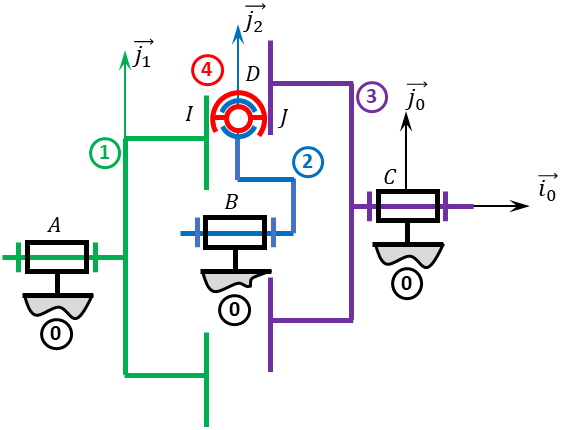
\includegraphics[width=\linewidth]{20_01}
\end{marginfigure}
\fi

\question{Tracer le graphe des liaisons.}
\ifprof
\else
\fi

\question{Déterminer la loi entrée -- sortie.}
\ifprof
\else
\fi


\ifprof
\else

\marginnote{Corrigé  voir \ref{TEC:05:C2:09:19}.}

\fi